\section{Model\-Car\-Dyn\-Rollover  Class Reference}
\label{classModelCarDynRollover}\index{ModelCarDynRollover@{Model\-Car\-Dyn\-Rollover}}
A car model considering the rolling effect and the pressure on different tires of the car is different. If the pressure on one tire is 0, the car is considered rolling over. The pressure model of the tire is rigid such that pressure can change at instant time, which means: (1) It might be the reason that only forward {\bf RRT} {\rm (p.\,\pageref{classRRT})} tree works. (2) In the Select\-Input function, pressure has to be restored when to test new inputs. 


{\tt \#include $<$modelcar.h$>$}

Inheritance diagram for Model\-Car\-Dyn\-Rollover::\begin{figure}[H]
\begin{center}
\leavevmode
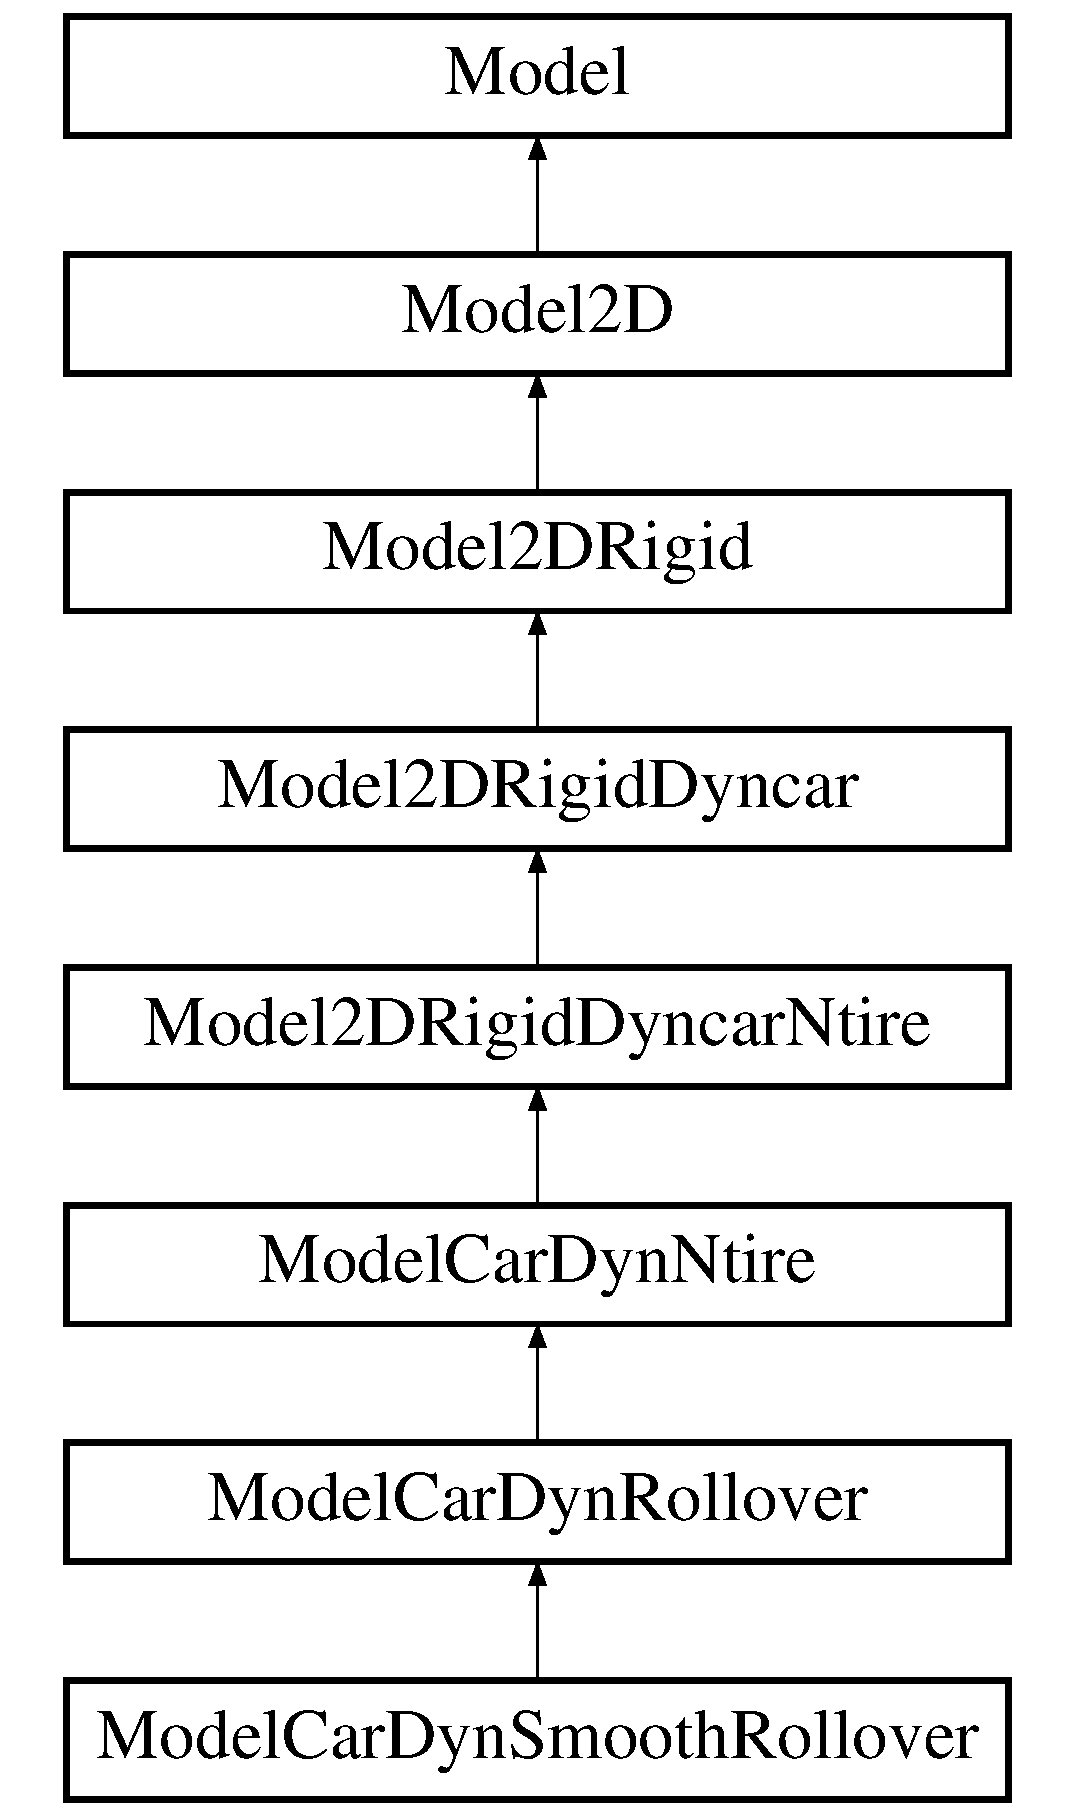
\includegraphics[height=8cm]{classModelCarDynRollover}
\end{center}
\end{figure}
\subsection*{Public Methods}
\begin{CompactItemize}
\item 
{\bf Model\-Car\-Dyn\-Rollover} (string path)
\item 
virtual {\bf $\sim$Model\-Car\-Dyn\-Rollover} ()
\item 
int {\bf sgn} (double {\bf x})
\item 
virtual {\bf MSLVector} {\bf State\-Transition\-Equation} (const {\bf MSLVector} \&x1, const {\bf MSLVector} \&u)
\begin{CompactList}\small\item\em The state transition equation, or equations of motion, xdot=f(x,u).\item\end{CompactList}\item 
virtual {\bf MSLVector} {\bf State\-To\-Configuration} (const {\bf MSLVector} \&{\bf x})
\begin{CompactList}\small\item\em A method that converts a {\bf Model} {\rm (p.\,\pageref{classModel})} state in to a {\bf Geom} {\rm (p.\,\pageref{classGeom})} configuration.\item\end{CompactList}\item 
virtual {\bf MSLVector} {\bf Integrate} (const {\bf MSLVector} \&{\bf x}, const {\bf MSLVector} \&u, const double \&h)
\begin{CompactList}\small\item\em !!!!!!!! It has both the state and the uncontrolled state.\item\end{CompactList}\item 
virtual double {\bf Metric} (const {\bf MSLVector} \&x1, const {\bf MSLVector} \&x2)
\begin{CompactList}\small\item\em A distance metric, which is Euclidean in the base class.\item\end{CompactList}\item 
bool {\bf Roll\-Over\-Free} (const {\bf MSLVector} \&{\bf x})
\item 
bool {\bf Satisfied} (const {\bf MSLVector} \&{\bf x})
\begin{CompactList}\small\item\em Test whether global state-space constraints are satisfied.\item\end{CompactList}\end{CompactItemize}
\subsection*{Public Attributes}
\begin{CompactItemize}
\item 
double {\bf K}
\item 
double {\bf c}
\item 
double {\bf Ixx}
\item 
double {\bf T}
\item 
double {\bf H}
\item 
double {\bf H2}
\item 
double {\bf Ms}
\item 
double {\bf Wn}
\item 
double {\bf Fai}
\item 
double {\bf x}
\item 
bool {\bf Is\-Roll\-Over}
\end{CompactItemize}


\subsection{Detailed Description}
A car model considering the rolling effect and the pressure on different tires of the car is different. If the pressure on one tire is 0, the car is considered rolling over. The pressure model of the tire is rigid such that pressure can change at instant time, which means: (1) It might be the reason that only forward {\bf RRT} {\rm (p.\,\pageref{classRRT})} tree works. (2) In the Select\-Input function, pressure has to be restored when to test new inputs.



\subsection{Constructor \& Destructor Documentation}
\index{ModelCarDynRollover@{Model\-Car\-Dyn\-Rollover}!ModelCarDynRollover@{ModelCarDynRollover}}
\index{ModelCarDynRollover@{ModelCarDynRollover}!ModelCarDynRollover@{Model\-Car\-Dyn\-Rollover}}
\subsubsection{\setlength{\rightskip}{0pt plus 5cm}Model\-Car\-Dyn\-Rollover::Model\-Car\-Dyn\-Rollover (string {\em path} = \char`\"{}\char`\"{})}\label{classModelCarDynRollover_a0}


\index{ModelCarDynRollover@{Model\-Car\-Dyn\-Rollover}!~ModelCarDynRollover@{$\sim$ModelCarDynRollover}}
\index{~ModelCarDynRollover@{$\sim$ModelCarDynRollover}!ModelCarDynRollover@{Model\-Car\-Dyn\-Rollover}}
\subsubsection{\setlength{\rightskip}{0pt plus 5cm}Model\-Car\-Dyn\-Rollover::$\sim$Model\-Car\-Dyn\-Rollover ()\hspace{0.3cm}{\tt  [inline, virtual]}}\label{classModelCarDynRollover_a1}




\subsection{Member Function Documentation}
\index{ModelCarDynRollover@{Model\-Car\-Dyn\-Rollover}!Integrate@{Integrate}}
\index{Integrate@{Integrate}!ModelCarDynRollover@{Model\-Car\-Dyn\-Rollover}}
\subsubsection{\setlength{\rightskip}{0pt plus 5cm}{\bf MSLVector} Model\-Car\-Dyn\-Rollover::Integrate (const {\bf MSLVector} \& {\em x}, const {\bf MSLVector} \& {\em u}, const double \& {\em h})\hspace{0.3cm}{\tt  [virtual]}}\label{classModelCarDynRollover_a5}


!!!!!!!! It has both the state and the uncontrolled state.



Reimplemented from {\bf Model2DRigid\-Dyncar} {\rm (p.\,\pageref{classModel2DRigidDyncar_a2})}.\index{ModelCarDynRollover@{Model\-Car\-Dyn\-Rollover}!Metric@{Metric}}
\index{Metric@{Metric}!ModelCarDynRollover@{Model\-Car\-Dyn\-Rollover}}
\subsubsection{\setlength{\rightskip}{0pt plus 5cm}double Model\-Car\-Dyn\-Rollover::Metric (const {\bf MSLVector} \& {\em x1}, const {\bf MSLVector} \& {\em x2})\hspace{0.3cm}{\tt  [virtual]}}\label{classModelCarDynRollover_a6}


A distance metric, which is Euclidean in the base class.



Reimplemented from {\bf Model\-Car\-Dyn\-Ntire} {\rm (p.\,\pageref{classModelCarDynNtire_a3})}.

Reimplemented in {\bf Model\-Car\-Dyn\-Smooth\-Rollover} {\rm (p.\,\pageref{classModelCarDynSmoothRollover_a4})}.\index{ModelCarDynRollover@{Model\-Car\-Dyn\-Rollover}!RollOverFree@{RollOverFree}}
\index{RollOverFree@{RollOverFree}!ModelCarDynRollover@{Model\-Car\-Dyn\-Rollover}}
\subsubsection{\setlength{\rightskip}{0pt plus 5cm}bool Model\-Car\-Dyn\-Rollover::Roll\-Over\-Free (const {\bf MSLVector} \& {\em x})}\label{classModelCarDynRollover_a7}


\index{ModelCarDynRollover@{Model\-Car\-Dyn\-Rollover}!Satisfied@{Satisfied}}
\index{Satisfied@{Satisfied}!ModelCarDynRollover@{Model\-Car\-Dyn\-Rollover}}
\subsubsection{\setlength{\rightskip}{0pt plus 5cm}bool Model\-Car\-Dyn\-Rollover::Satisfied (const {\bf MSLVector} \& {\em x})\hspace{0.3cm}{\tt  [virtual]}}\label{classModelCarDynRollover_a8}


Test whether global state-space constraints are satisfied.



Reimplemented from {\bf Model} {\rm (p.\,\pageref{classModel_a4})}.\index{ModelCarDynRollover@{Model\-Car\-Dyn\-Rollover}!StateToConfiguration@{StateToConfiguration}}
\index{StateToConfiguration@{StateToConfiguration}!ModelCarDynRollover@{Model\-Car\-Dyn\-Rollover}}
\subsubsection{\setlength{\rightskip}{0pt plus 5cm}{\bf MSLVector} Model\-Car\-Dyn\-Rollover::State\-To\-Configuration (const {\bf MSLVector} \& {\em x})\hspace{0.3cm}{\tt  [virtual]}}\label{classModelCarDynRollover_a4}


A method that converts a {\bf Model} {\rm (p.\,\pageref{classModel})} state in to a {\bf Geom} {\rm (p.\,\pageref{classGeom})} configuration.



Reimplemented from {\bf Model\-Car\-Dyn\-Ntire} {\rm (p.\,\pageref{classModelCarDynNtire_a2})}.

Reimplemented in {\bf Model\-Car\-Dyn\-Smooth\-Rollover} {\rm (p.\,\pageref{classModelCarDynSmoothRollover_a3})}.\index{ModelCarDynRollover@{Model\-Car\-Dyn\-Rollover}!StateTransitionEquation@{StateTransitionEquation}}
\index{StateTransitionEquation@{StateTransitionEquation}!ModelCarDynRollover@{Model\-Car\-Dyn\-Rollover}}
\subsubsection{\setlength{\rightskip}{0pt plus 5cm}{\bf MSLVector} Model\-Car\-Dyn\-Rollover::State\-Transition\-Equation (const {\bf MSLVector} \& {\em x1}, const {\bf MSLVector} \& {\em u})\hspace{0.3cm}{\tt  [virtual]}}\label{classModelCarDynRollover_a3}


The state transition equation, or equations of motion, xdot=f(x,u).



Reimplemented from {\bf Model2DRigid\-Dyncar\-Ntire} {\rm (p.\,\pageref{classModel2DRigidDyncarNtire_a2})}.

Reimplemented in {\bf Model\-Car\-Dyn\-Smooth\-Rollover} {\rm (p.\,\pageref{classModelCarDynSmoothRollover_a2})}.\index{ModelCarDynRollover@{Model\-Car\-Dyn\-Rollover}!sgn@{sgn}}
\index{sgn@{sgn}!ModelCarDynRollover@{Model\-Car\-Dyn\-Rollover}}
\subsubsection{\setlength{\rightskip}{0pt plus 5cm}int Model\-Car\-Dyn\-Rollover::sgn (double {\em x})}\label{classModelCarDynRollover_a2}




\subsection{Member Data Documentation}
\index{ModelCarDynRollover@{Model\-Car\-Dyn\-Rollover}!Fai@{Fai}}
\index{Fai@{Fai}!ModelCarDynRollover@{Model\-Car\-Dyn\-Rollover}}
\subsubsection{\setlength{\rightskip}{0pt plus 5cm}double Model\-Car\-Dyn\-Rollover::Fai}\label{classModelCarDynRollover_m8}


\index{ModelCarDynRollover@{Model\-Car\-Dyn\-Rollover}!H@{H}}
\index{H@{H}!ModelCarDynRollover@{Model\-Car\-Dyn\-Rollover}}
\subsubsection{\setlength{\rightskip}{0pt plus 5cm}double Model\-Car\-Dyn\-Rollover::H}\label{classModelCarDynRollover_m4}


\index{ModelCarDynRollover@{Model\-Car\-Dyn\-Rollover}!H2@{H2}}
\index{H2@{H2}!ModelCarDynRollover@{Model\-Car\-Dyn\-Rollover}}
\subsubsection{\setlength{\rightskip}{0pt plus 5cm}double Model\-Car\-Dyn\-Rollover::H2}\label{classModelCarDynRollover_m5}


\index{ModelCarDynRollover@{Model\-Car\-Dyn\-Rollover}!IsRollOver@{IsRollOver}}
\index{IsRollOver@{IsRollOver}!ModelCarDynRollover@{Model\-Car\-Dyn\-Rollover}}
\subsubsection{\setlength{\rightskip}{0pt plus 5cm}bool Model\-Car\-Dyn\-Rollover::Is\-Roll\-Over}\label{classModelCarDynRollover_m10}


\index{ModelCarDynRollover@{Model\-Car\-Dyn\-Rollover}!Ixx@{Ixx}}
\index{Ixx@{Ixx}!ModelCarDynRollover@{Model\-Car\-Dyn\-Rollover}}
\subsubsection{\setlength{\rightskip}{0pt plus 5cm}double Model\-Car\-Dyn\-Rollover::Ixx}\label{classModelCarDynRollover_m2}


\index{ModelCarDynRollover@{Model\-Car\-Dyn\-Rollover}!K@{K}}
\index{K@{K}!ModelCarDynRollover@{Model\-Car\-Dyn\-Rollover}}
\subsubsection{\setlength{\rightskip}{0pt plus 5cm}double Model\-Car\-Dyn\-Rollover::K}\label{classModelCarDynRollover_m0}


\index{ModelCarDynRollover@{Model\-Car\-Dyn\-Rollover}!Ms@{Ms}}
\index{Ms@{Ms}!ModelCarDynRollover@{Model\-Car\-Dyn\-Rollover}}
\subsubsection{\setlength{\rightskip}{0pt plus 5cm}double Model\-Car\-Dyn\-Rollover::Ms}\label{classModelCarDynRollover_m6}


\index{ModelCarDynRollover@{Model\-Car\-Dyn\-Rollover}!T@{T}}
\index{T@{T}!ModelCarDynRollover@{Model\-Car\-Dyn\-Rollover}}
\subsubsection{\setlength{\rightskip}{0pt plus 5cm}double Model\-Car\-Dyn\-Rollover::T}\label{classModelCarDynRollover_m3}


\index{ModelCarDynRollover@{Model\-Car\-Dyn\-Rollover}!Wn@{Wn}}
\index{Wn@{Wn}!ModelCarDynRollover@{Model\-Car\-Dyn\-Rollover}}
\subsubsection{\setlength{\rightskip}{0pt plus 5cm}double Model\-Car\-Dyn\-Rollover::Wn}\label{classModelCarDynRollover_m7}


\index{ModelCarDynRollover@{Model\-Car\-Dyn\-Rollover}!c@{c}}
\index{c@{c}!ModelCarDynRollover@{Model\-Car\-Dyn\-Rollover}}
\subsubsection{\setlength{\rightskip}{0pt plus 5cm}double Model\-Car\-Dyn\-Rollover::c}\label{classModelCarDynRollover_m1}


\index{ModelCarDynRollover@{Model\-Car\-Dyn\-Rollover}!x@{x}}
\index{x@{x}!ModelCarDynRollover@{Model\-Car\-Dyn\-Rollover}}
\subsubsection{\setlength{\rightskip}{0pt plus 5cm}double Model\-Car\-Dyn\-Rollover::x}\label{classModelCarDynRollover_m9}




The documentation for this class was generated from the following files:\begin{CompactItemize}
\item 
{\bf modelcar.h}\item 
{\bf modelcar.C}\end{CompactItemize}
